\section{区域积分的定义与性质}
\label{sec:multivariable-region-integration}

一块不均匀的金属薄片占据平面区域$D$，在点$(x,y)$附近每单位面积的质量为$\rho(x,y)$。
把$D$切成许多小块，每块的质量约等于块内某一点的密度乘这块的面积；把所有小块的质量相加，就得到总质量的近似值，小块切得越细，近似越准确。
空间物体的质量、带电体的总电荷也按同样方式累计，只是面积换成体积，面密度换成体密度或电荷密度。
这类问题中的被积函数都是多元标量函数$f:D\subseteq\mathbb R^d\to\mathbb R$：输入是一个位置的$d$个坐标，输出是该位置上一个待累计的数。

同一个积分还有两种常用读法。
若$f\geq0$定义在平面区域$D$上，积分等于以$D$为底、以$f$的图像为顶的立体的体积，这是一元积分“曲线下方面积”在高一维的对应。
当$D$的面积有限且非零时，把积分除以面积，所得的数是$f$在$D$上的平均值，例如一个地区的平均降雨量或一块薄板的平均温度。

本章从有界区域上的Riemann积分出发。先定义分割与累计，再用截面、坐标变换和参数求导组织计算。一般可测函数与积分极限定理在\BookChapterRef{chap:integration}{第~\ref{chap:integration}章}中建立，这里不以它们为前提。

\subsection{盒体积与Jordan区域}

闭坐标盒$Q=\prod_{j=1}^d[a_j,b_j]$的体积定义为$\operatorname{vol}(Q)=\prod_j(b_j-a_j)$。某条边长度为零时体积为零。

沿任意坐标把盒切成有限块，切开的边长相加仍等于原边长，因此小盒体积之和等于原体积；对有限网格反复应用便得到有限可加性，公共的盒边界不重复贡献体积。

对有界集合$D\subset\mathbb R^d$，用有限个内部互不相交的盒从内侧和外侧逼近$D$。若每个$\varepsilon>0$都能选取这样的内、外有限盒并，使外侧总体积与内侧总体积之差小于$\varepsilon$，称$D$为Jordan可测集合。这个共同逼近的极限称为$D$的Jordan体积，记为$|D|$。

体积不依赖所选网格：任取一组内逼近和另一组外逼近，前者体积不超过后者；当两侧差距可任意小时，能够夹住的数只有一个。

有界集合Jordan可测的等价条件是：其边界$\partial D$可被有限个总体积任意小的盒覆盖。边界以外的点或者有邻域完全落在$D$内，或者有邻域完全落在$D$外；因此同时接触$D$和其补集的网格小盒必与边界相交。

给定$\varepsilon>0$，先用有限个总体积小于$\varepsilon/2$的盒覆盖边界，再将每个盒的各边稍微向外扩张，使扩张后总体积仍小于$\varepsilon$。因为盒的个数有限，可选足够小的网格直径，使每个与边界相交的小盒都落入某个扩张盒。小盒内部互不重叠，故这些小盒的体积之和至多为扩张盒总体积，小于$\varepsilon$。

反过来，边界包含在外逼近减去内逼近的内部之后所剩的部分中；这部分除内外体积之差外，至多还包含有限个盒的边界。盒边界同样可用总体积任意小的有限盒覆盖，所以整个边界可被任意小体积覆盖。这一条件也解释了边界为何不影响累计：只要被积函数有界，落在边界附近的总贡献就被函数绝对值上界乘覆盖盒总体积控制。

例如闭圆盘是Jordan可测的。它的圆周可以分成有限条足够短的弧，每条弧用小正方形覆盖；当弧长尺度缩小时，所需正方形个数按尺度的倒数增长，而每个正方形面积按尺度的平方缩小，所以总面积趋于零。同理，有限条分片光滑曲线围成的平面区域，以及有限片光滑曲面围成的有界立体，其边界都能这样覆盖。这里依赖有限片及其足够规则的参数化，不能仅凭“看起来像曲线或曲面”就忽略任意复杂边界。

\subsection{多元Riemann和与可积性}

设$R$是包含$D$的闭坐标盒。沿各坐标作有限分割，得到小盒$Q_1,\ldots,Q_N$；网格大小是各小盒直径的最大值。在每个$Q_i$中任选取样点$\bm\xi_i$，对$R$上的有界函数$g$形成Riemann和
\[
 S(g,P,\bm\xi)=\sum_{i=1}^N g(\bm\xi_i)\operatorname{vol}(Q_i).
\]
若当网格大小趋于零时，不论如何选取分割和取样点，这些和都趋于同一个有限值，就称$g$在$R$上Riemann可积，公共极限记作$\int_R g(\bm x)\,\mathrm d\bm x$。

这一要求控制所有足够细的取样，而不是只检查某一种选点方式。

在每个小盒上分别取函数的上确界和下确界，乘盒体积并求和，得到上和$U(g,P)$和下和$L(g,P)$。任意取样和都位于二者之间；$g$可积当且仅当可以通过足够细的分割使$U(g,P)-L(g,P)$任意小。

若$g$在$R$上连续，紧性保证它一致连续；网格足够细时，每个小盒上的最大与最小函数值相差任意小，上下和的差便不超过这个差值乘$R$的体积，因此$g$可积。

对于有界Jordan可测的$D$和$D$上的有界函数$f$，令$g=f\mathbb I_D$，即在$R\setminus D$上取零。若$g$在$R$上Riemann可积，就把其积分定义为$\int_D f$。选择更大的包含盒只增加一片零延拓区域，不改变结果。

若$f$可以连续延拓到$\overline D$，则该延拓在闭包上一致连续。远离边界的小盒可用一致连续性控制振幅，靠近边界的小盒由前述有限盒覆盖控制总体积，所以零延拓可积。有限分块上分别连续、且不连续只落在这些分块可忽略边界上的有界函数，也可逐块使用同一论证。边界上怎样赋值不改变积分。

连续只是充分条件，不是必要条件。例如$R=[0,1]^2$上令$g(x,y)=\mathbb I_{\{x\geq1/2\}}$，它在直线$x=1/2$上不连续，但只有穿过该直线的网格小盒可能贡献上下和差；这些小盒的总面积随网格变细趋于零，因此$g$可积，其积分为$1/2$。

相反，有界本身不够：$\mathbb I_{\mathbb Q^2}$在每个非退化小盒内既取$0$也取$1$，上下和之差始终等于盒体积，因而不可积。

\subsection{积分的性质与累计量}

线性、单调性和绝对值估计都由有限Riemann和的对应性质取极限得到。例如若$f$、$h$可积且$f\leq h$，则$\int_D f\leq\int_D h$，并且$|\int_D f|\leq\int_D|f|$。有限个Jordan区域内部互不重叠，且拼接处落在可忽略的公共边界上时，分别求和再相加，得到区域可加性。

取$f=1$得到体积；非负密度$\rho$的积分是总质量，$|D|>0$时$|D|^{-1}\int_D f$是平均值；质量$M=\int_D\rho$有限且非零时，质心为$M^{-1}\int_D\bm x\rho(\bm x)\,\mathrm d\bm x$，向量积分按分量计算。

\section{累次积分}

区域积分的定义把所有坐标同时分割；计算时希望先沿一个方向累计，再沿其他方向累计。能否这样做，需要同时控制各截面的误差。

\subsection{长方体上的累次积分}

设$f$在闭矩形$R=[a,b]\times[c,d]$上连续。固定$x$时，一元积分$F(x)=\int_c^d f(x,y)\,\mathrm dy$存在。由于$f$在$R$上一致连续，当$x$变化足够小时，所有$y\in[c,d]$处的函数值同时变化很小，故$F$连续。

对乘积网格，把有限个取样和按列分组；内层求和趋于各列的$y$方向积分，一致连续性控制所有列的误差，外层求和再趋于$\int_a^bF(x)\,\mathrm dx$。按行分组同理，因而
\[
 \int_R f(x,y)\,\mathrm d(x,y)
 =\int_a^b\left(\int_c^d f(x,y)\,\mathrm dy\right)\mathrm dx
 =\int_c^d\left(\int_a^b f(x,y)\,\mathrm dx\right)\mathrm dy.
\]
这是一组容易核对的充分条件：一般Riemann可积函数的每个截面未必都可积，不能仅由整体可积就不检查内层积分。更多坐标的闭盒可重复上述分组。

\subsection{简单区域与积分次序的选择}

若$D=\{(x,y):a\leq x\leq b,\ \alpha(x)\leq y\leq\beta(x)\}$，边界函数$\alpha\leq\beta$连续，且$f$在$D$的闭包上连续，则
\[
 \int_D f(x,y)\,\mathrm d(x,y)
 =\int_a^b\left(\int_{\alpha(x)}^{\beta(x)}f(x,y)\,\mathrm dy\right)\mathrm dx.
\]
这是对零延拓作网格分组：边界曲线附近的格子总体积可任意小，其余格子按截面累计。连续边界与紧性保证截面端点随$x$一致变化，内层积分也随$x$连续。有限个这样的区域可逐块处理，公共边界不重复累计；换次序时须重新求出投影和截面。

例如$D=\{0\leq y\leq x\leq1\}$，取$f(x,y)=x+y$。固定$x$，截面为$0\leq y\leq x$，得到
\[
 \int_0^1\left(\int_0^x(x+y)\,\mathrm dy\right)\mathrm dx
 =\int_0^1\frac{3x^2}{2}\,\mathrm dx=\frac12.
\]
固定$y$时截面变为$y\leq x\leq1$，因此同一个量也等于
\[
 \int_0^1\left(\int_y^1(x+y)\,\mathrm dx\right)\mathrm dy
 =\int_0^1\left(\frac12+y-\frac{3y^2}{2}\right)\mathrm dy=\frac12.
\]
两个上下限来自同一三角形的不同截面，并不是把原积分符号机械交换。

换序还可能改变分块方式。例如区域$0\leq x\leq2$、$0\leq y\leq\min(x,2-x)$是一个三角形。先对$y$积分时，在$x=1$处分成两块；先对$x$积分则用$0\leq y\leq1$、$y\leq x\leq2-y$。以$f=1$核验，两种次序都给出面积$1$。上下限来自截面，而不是积分符号本身。

\subsection{截断、奇点与交换次序的边界}

无界区域或无界密度不能直接代入上面的有界Riemann和。可以先选一族有界Jordan区域$D_\varepsilon$，避开奇点或截去远处，并逐个检查$f$在每个截断区域上Riemann可积，再考察$\int_{D_\varepsilon}f$的极限。

只沿某一族截断得到极限，并不自动证明其他截断方式给出相同结果。

例如在$(0,1]^2$上取$f(x,y)=(x^2-y^2)/(x^2+y^2)^2$。对$0<\varepsilon<1$，先用$D_\varepsilon=[\varepsilon,1]\times[\varepsilon^2,1]$截断。每个截断矩形远离原点，$f$连续。

若暂把下边界改为$y=0$，先对$y$积分可得
\[
 \int_\varepsilon^1\left(\int_0^1 f(x,y)\,\mathrm dy\right)\mathrm dx
 =\int_\varepsilon^1\frac{\mathrm dx}{1+x^2}
 \longrightarrow\frac\pi4.
\]
被去掉的窄条上$|f(x,y)|\leq1/x^2$，其绝对积分不超过$\varepsilon^2\int_\varepsilon^1x^{-2}\,\mathrm dx\to0$，故$\int_{D_\varepsilon}f\to\pi/4$。交换两条边的截断速度，令$E_\varepsilon=[\varepsilon^2,1]\times[\varepsilon,1]$；由$f(y,x)=-f(x,y)$，所得极限是$-\pi/4$。两族矩形都逐渐填满同一区域$(0,1]^2$，却得到不同极限；因此这里没有与这两种截断方式无关的总量。


\section{区域积分的换元}
\label{sec:classical-change-variables}

圆盘用半径和角度描述比用两个直角坐标更简单。但坐标变化也会改变小块的面积或体积，不能只替换函数中的变量。前面已经知道线性映射把体积乘以行列式的绝对值；可微映射在足够小的区域内近似线性，换元公式正是把这些局部比例累计起来。

\subsection{局部体积变化与换元公式}

为了明确单次覆盖和边界条件，先在两个开集之间使用可微双射，再取其中的有界积分区域。
\begin{theorem}[经典区域积分的换元]
设$U,V\subseteq\mathbb R^d$为开集，$T:U\to V$为$C^1$双射，逆映射也为$C^1$。设$E\subset U$为紧Jordan区域，且$T(E)$也是Jordan区域。若$f$在$T(E)$上连续，则
\[
 \int_{T(E)}f(\bm x)\,\mathrm d\bm x
 =\int_E f(T(\bm u))|\det DT(\bm u)|\,\mathrm d\bm u.
\]
\end{theorem}

先说明公式中的权重。对$E$附近等边网格中的小立方体，连续可微性给出统一的一阶近似
\[
 T(\bm u+\bm h)-T(\bm u)=DT(\bm u)\bm h+\bm R_{\bm u}(\bm h).
\]
当$\|\bm h\|\leq\delta$时，余项满足$\|\bm R_{\bm u}(\bm h)\|\leq\eta(\delta)\|\bm h\|$，其中$\eta(\delta)\to0$，并且这个界在紧集上对$\bm u$一致。逆导数同样有界，所以局部小盒不会在某一方向被任意压扁。

在线性像平行多面体的边界外加厚度与$\eta(\delta)\delta$同阶的薄层，就能夹住小盒的像；薄层体积相对于原盒体积趋于零。这给出局部体积比趋于$|\det DT(\bm u)|$。把像分割上的取样和与参数小盒上的加权取样和比较，连续函数的一致连续性控制函数值替换误差，前述统一余项控制体积误差，Jordan边界条件控制边界小块，取极限得到公式。

这是证明的局部分割思路；仅写出某一点的线性近似，尚不足以交换整个分割和的极限。

逆函数定理只保证每一点附近可以反解，并不保证整个区域只覆盖一次。上面的全局双射条件正是防止重复累计；行列式绝对值消除的是定向符号，不能消除覆盖次数。

\subsection{极坐标、柱坐标与球坐标}

平面极坐标将$(r,\theta)$送到$(r\cos\theta,r\sin\theta)$，Jacobian行列式为$r$。同一角度宽度在半径较大处扫过更长的弧，所以参数矩形的面积不能直接当作平面小块的面积。其面积权重是
\[
 \mathrm dA=r\,\mathrm dr\,\mathrm d\theta.
\]

\begin{figure}[!htb]
\centering
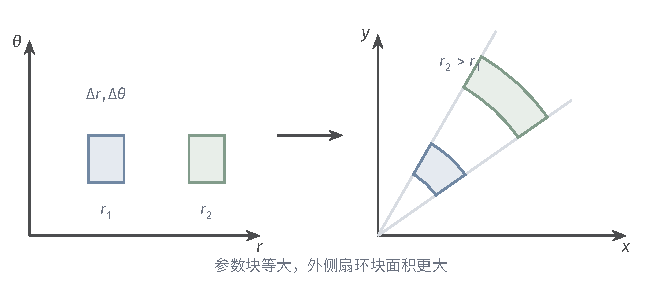
\includegraphics[width=112mm]{figures/00-shared/mathematical-preliminaries-upper/00-shared/tikz/mathematical-language-combinatorics-analysis-optimization-comprehension-additions/polar-area-weight.pdf}
\caption{同样的径向宽度和角度宽度，在较大半径处产生更大的面积。一阶面积为$r\Delta r\Delta\theta$，由此得到极坐标权重。}
\label{fig:vol3-classical-polar-weight}
\end{figure}

原点处行列式为零，角度的两端又表示同一条射线，因此不能把闭参数矩形直接代入上述双射定理。可以先限制$r\geq\varepsilon$且$\varepsilon\leq\theta\leq2\pi-\varepsilon$，在紧截断区域上换元，再令$\varepsilon\downarrow0$。对于圆盘上的连续函数，被去掉的小圆盘和窄扇区的贡献受函数上界乘面积控制，趋于零；参数侧的遗漏也由有界权重控制。

例如半径$R$的圆盘面积为
\[
 \int_0^{2\pi}\int_0^R r\,\mathrm dr\,\mathrm d\theta=\pi R^2.
\]
若角度取到$4\pi$，内部被覆盖两次，结果也变成两倍。对于有奇点的被积函数，不能只用“接缝不贡献面积”来跳过极限估计。

柱坐标保留高度$z$，即在极坐标后加上第三个坐标，其体积权重仍含$r$：
\[
 \mathrm dV=r\,\mathrm dr\,\mathrm d\theta\,\mathrm dz.
\]
因此半径$R$、高度$H$的圆柱体积为$\pi R^2H$。轴线和角度接缝通过与极坐标相同的截断处理。

球坐标使用距原点的距离$\rho$、从正$z$轴量起的极角$\varphi$和方位角$\theta$：
\[
 T(\rho,\varphi,\theta)
 =(\rho\sin\varphi\cos\theta,\rho\sin\varphi\sin\theta,\rho\cos\varphi).
\]
三个局部正交方向的长度比例分别是$1$、$\rho$和$\rho\sin\varphi$，也可直接计算Jacobian行列式验证。因此
\[
 \mathrm dV=\rho^2\sin\varphi\,\mathrm d\rho\,\mathrm d\varphi\,\mathrm d\theta.
\]

在$\rho>0$、$0<\varphi<\pi$及一个长度为$2\pi$的开角度区间内，映射单次覆盖去掉轴线和接缝后的空间。计算球内连续函数的积分时，先截去原点、极轴附近及接缝附近的小区域，再以有界性估计遗漏。球体积由此为
\[
 \int_0^{2\pi}\int_0^\pi\int_0^R
 \rho^2\sin\varphi\,\mathrm d\rho\,\mathrm d\varphi\,\mathrm d\theta
 =\frac{4\pi R^3}{3}.
\]

\subsection{线性换元与积分结果的核对}

线性变换可以把斜区域变成坐标盒。

设$D$由$0\leq x+y\leq2$和$0\leq x-y\leq2$围成，求$\int_D(x+y)\,\mathrm d(x,y)$。令$u=x+y$、$v=x-y$，则参数区域为$[0,2]^2$，逆变换为
\[
 x=(u+v)/2,
\]
\[
 y=(u-v)/2.
\]
其行列式为$-1/2$，故面积权重为$1/2$。于是
\[
 \int_D(x+y)\,\mathrm d(x,y)
 =\int_0^2\int_0^2\frac u2\,\mathrm du\,\mathrm dv=2.
\]
取被积函数为$1$，同样得到区域面积$2$；原被积函数在对称区域上的平均值为$1$，两者相乘也为$2$。这同时核验了区域、权重和积分值。

\section{参数积分}

若密度或被积函数还依赖一个参数，积分便定义了新的函数。

判断它是否连续、能否求导，需要控制整个积分区域上的变化，逐点成立的极限本身不够。本节固定紧Jordan区域$D$，用连续性提供统一控制。

\subsection{固定区域上的参数积分与连续性}

设$K$为紧参数区域，$f$在$D\times K$上连续，记
\[
 F(\bm t)=\int_D f(\bm x,\bm t)\,\mathrm d\bm x.
\]
乘积紧集上的一致连续性使$\sup_{\bm x\in D}|f(\bm x,\bm t)-f(\bm x,\bm s)|$在$\bm t\to\bm s$时趋于零。因此
\[
 |F(\bm t)-F(\bm s)|
 \leq |D|\sup_{\bm x\in D}|f(\bm x,\bm t)-f(\bm x,\bm s)|\longrightarrow0.
\]
这证明了连续性。参数区域不必整体有界：讨论一个内点附近时，取包含该点的小闭盒即可。

\subsection{积分号下的偏导数与全微分}

现在设参数属于开集，$f$和各参数偏导$\partial_{t_j}f$在$D$与参数邻域的乘积上连续。固定一个参数点和足够小的闭邻域，一元中值定理把差商写成附近参数处的偏导值。偏导的一致连续性说明差商对全部$\bm x\in D$一致趋于$\partial_{t_j}f$；对差取积分并用上面的上确界估计，便得到
\begin{equation}
 \partial_{t_j}F(\bm t)=\int_D\partial_{t_j}f(\bm x,\bm t)\,\mathrm d\bm x.
\label{eq:classical-differentiate-under-integral}
\end{equation}
右侧又是连续参数积分，故所有参数偏导连续，$F$是$C^1$函数。它的全微分为
\[
 DF_{\bm t}[\bm h]=\int_D D_{\bm t}f(\bm x,\bm t)[\bm h]\,\mathrm d\bm x.
\]

这里先获得偏导，再由连续偏导判据得到整体可微；不能只证明每个方向上的极限就略去这一步。

例如$F(t)=\int_0^1 e^{tx}\,\mathrm dx$，在任意有界参数区间上都满足这些条件，故$F'(0)=\int_0^1x\,\mathrm dx=1/2$，无需在$t=0$处处理显式表达式的可去奇点。

\subsection{变限参数积分}

积分区间也随参数变化时，积分值的变化有两部分：原区间内部函数改变，以及两端新添或移除的细条。

设$a(t),b(t)$为$C^1$函数，$f(x,t)$及$\partial_tf(x,t)$在所需区间附近连续。将积分写为固定基点到$b(t)$的积分减去固定基点到$a(t)$的积分，再用链式法则，得到
\[
 \frac{\mathrm d}{\mathrm dt}\int_{a(t)}^{b(t)}f(x,t)\,\mathrm dx
 =\int_{a(t)}^{b(t)}\partial_tf(x,t)\,\mathrm dx
 +f(b(t),t)b'(t)-f(a(t),t)a'(t).
\]

上端向右移动增加积分，下端向右移动减少积分，所以两个边界项符号相反。多个参数时逐一求偏导，或将$a'$、$b'$和$\partial_tf$换成作用于同一参数增量的全微分。更一般的移动区域会产生沿边界的贡献；本章只在上述区间变限和已明确参数化的区域上使用这一规则。
